\documentclass[a4paper, 12pt]{article}
\usepackage[a4paper,top=1.5cm, bottom=1.5cm, left=1cm, right=1cm]{geometry}
\usepackage[utf8]{inputenc}
\usepackage{amsmath}
\usepackage{amssymb}
\usepackage{amsfonts}
\usepackage[english, russian]{babel}
\usepackage{indentfirst}
\usepackage{longtable}
\usepackage{graphicx}

\usepackage{float}
\restylefloat{table}

\title{Лабораторная работа 2.1.6\\ Эффект Джоуля-Томсона}
\author{Симанкович Александр \\ Б01-104}
\date{15.02.2021}

\begin{document}
	\maketitle
	
	\section*{Цель работы} 
	1) Определение изменения температуры углекислого газа при протекании через малопроницаемую перегородку при разных начальных значениях давления и температуры;
	
	2) Вычисление по результатам опытов коэффициентов Ван-дер-Ваальса $'a'$ и $'b'$.
	
	\section*{Оборудование и приборы} Трубка с пористой перегородкой; труба Дьюара; термостат; термометры; дифференциальная термопара; микровольтметр; балластный баллон; манометр.
	
\section*{Теоретическое введение}
Эффектом Джоуля–Томсона называется изменение температуры газа, медленно протекающего из области высокого в область низкого давления в условиях хорошей тепловой изоляции. В разреженных газах, которые приближаются по своим свойствам к идеальному газу, при таком течении температура газа не меняется. Эффект Джоуля–Томсона демонстрирует отличие исследуемого газа от идеального.

В работе исследуется изменение температуры углекислого газа при медленном его течении по трубке с пористой перегородкой (риc. \ref{scheme}). Трубка 1 хорошо теплоизолирована. Величина эффекта Джоуля–Томсона определяется по разности температуры газа до и после перегородки.

Рассмотрим стационарный поток газа между произвольными сечениями I и II трубки. Пусть, для определенности, через трубку прошел 1 моль углекислого газа; $ \mu $ -- его молярная масса. Молярные объемы газа, его давления и отнесенные к молю внутренние энергии газа в сечениях I и II обозначим соответственно $ V_1, P_1, U_1 $ и $ V_2, P_2, U_2 $. Для того чтобы ввести в трубку объем $ V_1 $, над газом нужно совершить работу $ A_1 = P_1V_1 $. Проходя через сечение II, газ сам совершает работу $ A_2 = P_2V_2 $. Так как через боковые стенки не происходит ни обмена теплом, ни передачи механической энергии, то

\begin{equation}\label{1}
	A_1-A_2=\left(U_2+\frac{\mu v_2^2}{2}\right) - \left(U_1 + \frac{\mu v_1^2}{2}\right).
\end{equation}

В уравнении \eqref{1} учтено изменение как внутренней (первые члены в скобках), так и кинетической (вторые члены в скобках) энергии газа. Подставляя в \eqref{1} написанные выражения для $ A_1 $ и $ A_2 $ и перегруппировывая члены, найдем

\begin{equation}\label{2}
	H_1-H_2=\left(U_1+P_1V_1\right) - \left(U_2 + P_2V_2\right) = \frac{1}{2} \mu \left(v^2_2-v^2_1\right).
\end{equation}

Сделаем несколько замечаний. Прежде всего отметим, что в процессе Джоуля–Томсона газ испытывает в пористой перегородке существенное трение, приводящее к ее нагреву. Потери энергии на нагрев трубки в начале процесса могут быть очень существенными и сильно искажают ход явления. После того как температура трубки установится и газ станет уносить с собой все выделенное им в пробке тепло, формула \eqref{1} становится точной, если, конечно, теплоизоляция трубки достаточно хороша и не происходит утечек тепла наружу через ее стенки.

Второе замечание связано с правой частью \eqref{2}. Процесс Джоуля–Томсона в чистом виде осуществляется лишь в том случае, если правой частью можно пренебречь, т. е. если макроскопическая скорость газа с обеих сторон трубки достаточно мала. У нас сейчас нет критерия, который позволил бы установить, когда это можно сделать. В силу сохранения энтропии в случае реального газа получаем:

\begin{equation}\label{3}
	\mu_\text{Д--Т} = \frac{\Delta T}{\Delta P} \approx \frac{\frac{2a}{RT} - b}{C_P}.
\end{equation}

Из формулы \eqref{3} видно, что эффект Джоуля–Томсона для не очень плотного газа зависит от соотношения величин $ a $ и $ b $, которые оказывают противоположное влияние на знак эффекта. Если силы взаимодействия между молекулами велики, так что превалирует <<поправка на давление>>, то основную роль играет член, содержащий $a$, и 

$$ \frac{\Delta T}{\Delta P} > 0, $$
т. е. газ при расширении охлаждается ($ \Delta T < 0 $, так как всегда $ \Delta P < 0 $). В обратном случае (малые $ a $)

$$ \frac{\Delta T}{\Delta P} < 0, $$
т. е. газ нагревается ($ \Delta T > 0 $, так как по-прежнему $ \Delta P < 0 $).

Этот результат нетрудно понять из энергетических соображений. Как мы уже знаем, у идеального газа эффект Джоуля–Томсона отсутствует. Идеальный газ отличается от реального тем, что в нем можно пренебречь потенциальной энергией взаимодействия молекул. Наличие этой энергии приводит к охлаждению или нагреванию реальных газов при расширении. При больших $a$ велика энергия притяжения молекул. Это означает, что потенциальная энергия молекул при их сближении уменьшается, а при удалении -- при расширении газа -- возрастает. Возрастание потенциальной энергии молекул происходит за счет их кинетической энергии -- температура газа при расширении падает. Аналогичные рассуждения позволяют понять, почему расширяющийся газ нагревается при больших значениях $b$.

Как следует из формулы \eqref{3}, при температуре \[ T_i = \frac{2a}{Rb} \] коэффициент $ \mu_\text{Д--Т} $ обращается в нуль. По формулам связи параметров газа Ван-дер-Ваальса с критическими параметрами получаем: 

\begin{equation}\label{4}
	T_\text{инв} = \frac{27}{4} T_\text{кр}.
\end{equation}

При температуре $ T_\text{инв} $ эффект Джоуля–Томсона меняет знак: ниже температуры инверсии эффект положителен ($ \mu_\text{Д--Т} > 0 $, газ охлаждается), выше $ T_\text{инв} $ эффект отрицателен ($ \mu_\text{Д--Т} < 0 $, газ нагревается).

Вернемся к влиянию правой части уравнения \eqref{2} на изменение температуры расширяющегося газа. Для этого сравним изменение температуры, происходящее вследствие эффекта Джоуля–Томсона, с изменением температуры, возникающим из-за изменения кинетической энергии газа. Увеличение кинетической энергии газа вызывает заметное и приблизительно одинаковое понижение его температуры как у реальных, так и у идеальных газов. Поэтому при оценках нет смысла пользоваться сложными формулами для газа Ван-дер-Ваальса.

Заменяя в формуле \eqref{2} $ U $ через $ C_VT $ и $ PV $ через $ RT $, найдем

$$ \left(R+C_V\right)\left(T_1-T_2\right)=\mu\left(v_2^2-v_1^2\right)/2 $$
или
$$ \Delta T = \frac{\mu}{2C_P}\left(v_2^2-v_1^2\right). $$

В условиях нашего опыта расход газа $ Q  $ на выходе из пористой перегородки не превышает $ 10 $ см$ ^3 $/с, а диаметр трубки равен 3 мм. Поэтому

$$ v_2<=\frac{4Q}{\pi d^2} = \frac{4\cdot\text{см}^3/\text{с}}{3,14\cdot(0,3)^2\text{ см}^2} \approx 140 \text{ см}/\text{с}. $$

Скорость $ v_1 $ газа у входа в пробку относится к скорости $ v_2 $ у выхода из нее как давление $ P_2 $ относится к $ P_1 $. В нашей установке $ P_1 = 4 $ атм, a $ P_2 = 1 $ атм, поэтому

$$ v_1=\frac{P_2}{P_1}v_2 = 35 \text{ см}/\text{с}. $$

Для углекислого газа $ \mu = 44 $ г/моль, $ C_P = 40 $ Дж/(моль·К); имеем

$$ \Delta T = \frac{\mu}{2C_P}\left(v_2^2-v_1^2\right) \approx 7\cdot10^{-4} \text{ K}. $$

Это изменение температуры ничтожно мало по сравнению с измеряемым эффектом (несколько градусов).

В данной лабораторной работе исследуется коэффициент дифференциального эффекта Джоуля–Томсона для углекислого газа. По экспериментальным результатам оценивается коэффициент теплового расширения, постоянные в уравнении Ван-дер-Ваальса и температура инверсии углекислого газа. Начальная температура газа $ T_1 $ задается термостатом. Измерения проводятся при четырех температурах: 20 $ ^\circ $C, 30 $ ^\circ $C, 40 $ ^\circ $C и 50 $ ^\circ $C.

\section*{Экспериментальная установка}

\begin{figure}[H]
	\begin{center}
		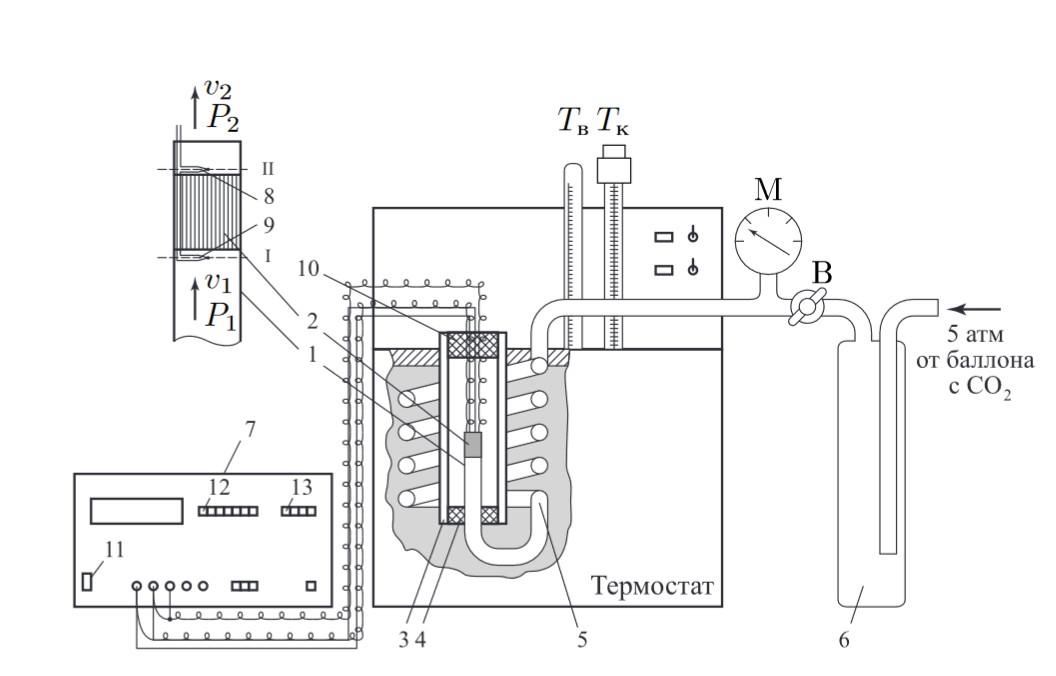
\includegraphics[width=18cm]{scheme.png}
	\end{center}
	\caption{\textit{Схема установки}}
	\label{scheme}
\end{figure}

Схема установки для исследования эффекта Джоуля–Томсона в углекислом газе представлена на рисунке \ref{scheme}. Основным элементом установки является трубка 1 с пористой перегородкой 2, через которую пропускается исследуемый газ. Трубка имеет длину 80 мм и сделана из нержавеющей стали, обладающей, как известно, малой теплопроводностью. Диаметр трубки $ d = 3 $~мм, толщина стенок 0,2 мм. Пористая перегородка расположена в конце трубки и представляет собой стеклянную пористую пробку со множеством узких и длинных каналов. Пористость и толщина пробки ($ l = 5 $ мм) подобраны так, чтобы обеспечить оптимальный поток газа при перепаде давлений $ \Delta P \leqslant 4 $ атм (расход газа составляет около $ 10 $ см$ ^3 $/с); при этом в результате эффекта Джоуля–Томсона создается достаточная разность температур.

Углекислый газ под повышенным давлением поступает в трубку через змеевик 5 из балластного баллона 6. Медный змеевик омывается водой и нагревает медленно протекающий через него газ до температуры воды в термостате. Температура воды измеряется термометром $ T_\text{в} $, помещенным в термостате. Требуемая температура воды устанавливается и поддерживается во время эксперимента при помощи контактного термометра $ T_\text{к} $.

Давление газа в трубке измеряется манометром М и регулируется вентилем В (при открывании вентиля В, т. е. при повороте ручки против часовой стрелки, давление $ P_1 $ повышается). Манометр М измеряет разность между давлением внутри трубки и наружным (атмосферным) давлением. Так как углекислый газ после пористой перегородки выходит в область с атмосферным давлением $ P_2 $, то этот манометр непосредственно измеряет перепад давления на входе и на выходе трубки $ \Delta P = P_1 - P_2 $.

Разность температур газа до перегородки и после нее измеряется дифференциальной термопарой медь -- константан. Константановая проволока диаметром 0,1 мм соединяет спаи 8 и 9, а медные проволоки (того же диаметра) подсоединены к цифровому вольтметру 7. Отвод тепла через проволоку столь малого сечения пренебрежимо мал. Для уменьшения теплоотвода трубка с пористой перегородкой помещена в трубу Дьюара 3, стенки которой посеребрены, для уменьшения теплоотдачи, связанной с излучением. Для уменьшения теплоотдачи за счет конвекции один конец трубы Дьюара уплотнен кольцом 4, а другой закрыт пробкой 10 из пенопласта. Такая пробка практически не создает перепада давлений между внутренней полостью трубы и атмосферой.

\section*{Ход работы}

	Приборные погрешности измерений:
	
	$$\sigma_U = 0.5 \; \text{мкВ} \;\;\; \sigma_{\Delta P} = 0.05 \; \text{атм} \;\;\; \sigma_T = 0.005 \; \text{K} \;\;\; \sigma_\alpha = 0.45 \; \frac{\text{мкВ}}{\text{К}}$$

	$$\sigma(\mu_{D-T})^{ \text{(сист)} } = \mu_{D-T} \cdot \sqrt{ 
		\Big(\frac{\sigma_U}{\overline{U}} \Big)^2 +
		\Big(\frac{\sigma_{\alpha}}{\alpha} \Big)^2 +
		\Big(\frac{\sigma_{\Delta P}}{\overline{\Delta P}} \Big)^2
	}$$
	
	Измерения проводились при четырех температурах: $T_1=293$K, $T_2=303$K, $T_3=313$K, $T_4=323$K. Для каждой температуры вычислим $\mu_{D-T}$.
	
	\begin{table}[H]
		\centering
		\begin{tabular}{llll}
			\hline
			\multicolumn{4}{c}{$T=293$ K ($20^\circ C$) $ \;\;\; \alpha = 40.0 \frac{\text{мкВ}}{\text{К}} $} \\
			\hline
			$\Delta P$, атм & $U$, мкВ & $\Delta T$, K & $T^{-1}$, $\text{K}^{-1}$ \\ \hline
			4.00        & 168      & 4.35  & 0.229            \\
			3.50      & 143      & 3.73  & 0.268            \\
			3.00         & 120      & 3.15  & 0.317            \\
			2.50       & 98       & 2.60  & 0.384            \\
			2.00         & 77       & 2.08  & 0.481            \\
			1.50       & 55       & 1.53  & 0.655            \\
			1.00         & 35       & 1.03  & 0.975            \\	\hline
		\end{tabular}
	\end{table}

	$$ \mu_{D-T} = 1.104 \; \text{K/атм} \;\;\; \sigma(\mu_{D-T})^{\text{случ}} = 0.016 \; \text{K/атм} $$

	$$ \sigma(\mu_{D-T})^{ \text{(сист)} } = 1.104 \cdot \sqrt{
		\Big(\frac{0.5}{105}\Big)^2 + 
		\Big(\frac{0.45}{40}\Big)^2 + 
		\Big(\frac{0.05}{2.5}\Big)^2
	} = 0.026 \; \text{K/атм} $$

	\begin{equation*}
		\mu_{D-T} = (1.10 \pm 0.04) \; \text{K/атм}
	\end{equation*}

	\begin{table}[H]
		\centering
		\begin{tabular}{llll}
			\hline
			\multicolumn{4}{c}{$T=303$ K ($30^\circ C$) $ \;\;\; \alpha = 41.0 \frac{\text{мкВ}}{\text{К}} $} \\
			\hline
			$\Delta P$, атм & $U$, мкВ & $\Delta T$, K & $T^{-1}$, $\text{K}^{-1}$ \\ \hline
			4.00 & 147 & 3.70 & 0.269 \\
			3.50 & 126 & 3.19 & 0.312 \\
			3.00 & 105 & 2.68 & 0.372 \\
			2.50 & 83  & 2.14 & 0.465 \\
			2.00 & 65  & 1.70 & 0.585 \\
			1.50 & 49  & 1.31 & 0.759 \\
			1.00 & 29  & 0.82 & 1.205 \\ 			\hline
		\end{tabular}
	\end{table}

	$$ \mu_{D-T} = 0.955 \; \text{K/атм} \;\;\; \sigma(\mu_{D-T})^{\text{случ}} = 0.020 \; \text{K/атм} $$
	
	$$ \sigma(\mu_{D-T})^{ \text{(сист)} } = 0.955 \cdot \sqrt{
		\Big(\frac{0.5}{91}\Big)^2 + 
		\Big(\frac{0.45}{41}\Big)^2 + 
		\Big(\frac{0.05}{2.5}\Big)^2
	} = 0.022 \; \text{K/атм} $$
	
	\begin{equation*}
		\mu_{D-T} = (0.96 \pm 0.04) \; \text{K/атм}
	\end{equation*}

	\begin{table}[H]
		\centering
		\begin{tabular}{llll}
			\hline
			\multicolumn{4}{c}{$T=313$ K ($40^\circ C$) $ \;\;\; \alpha = 42.0 \frac{\text{мкВ}}{\text{К}} $} \\
			\hline
			$\Delta P$, атм & $U$, мкВ & $\Delta T$, K & $T^{-1}$, $\text{K}^{-1}$ \\ \hline
			4.00 & 128 & 3.16 & 0.315 \\
			3.50 & 108 & 2.69 & 0.371 \\
			3.00 & 86  & 2.16 & 0.461 \\
			2.50 & 68  & 1.73 & 0.575 \\
			2.00 & 50  & 1.30 & 0.763 \\
			1.50 & 34  & 0.92 & 1.076 \\
			1.00 & 20  & 0.59 & 1.680 \\				\hline
		\end{tabular}
	\end{table}

	$$ \mu_{D-T} = 0.864 \; \text{K/атм} \;\;\; \sigma(\mu_{D-T})^{\text{случ}} = 0.027 \; \text{K/атм} $$
	
	$$ \sigma(\mu_{D-T})^{ \text{(сист)} } = 0.864 \cdot \sqrt{
		\Big(\frac{0.5}{75}\Big)^2 + 
		\Big(\frac{0.45}{42}\Big)^2 + 
		\Big(\frac{0.05}{2.5}\Big)^2
	} = 0.020 \; \text{K/атм} $$

	\begin{equation*}
		\mu_{D-T} = (0.86 \pm 0.05) \; \text{K/атм}
	\end{equation*}
	
	\begin{table}[H]
		\centering
		\begin{tabular}{llll}
			\hline
			\multicolumn{4}{c}{$T=323$ K ($50^\circ C$) $ \;\;\; \alpha = 43.0 \frac{\text{мкВ}}{\text{К}} $} \\
			\hline
			$\Delta P$, атм & $U$, мкВ & $\Delta T$, K & $T^{-1}$, $\text{K}^{-1}$ \\ \hline
			4.00 & 101 & 2.46 & 0.405 \\
			3.50 & 82  & 2.02 & 0.494 \\
			3.00 & 62  & 1.55 & 0.641 \\
			2.50 & 47  & 1.20 & 0.826 \\
			2.00 & 36  & 0.95 & 1.048 \\
			1.50 & 26  & 0.72 & 1.387 \\
			1.00 & 16  & 0.48 & 2.047 \\				\hline
		\end{tabular}
	\end{table}

	$$ \mu_{D-T} = 0.653 \; \text{K/атм} \;\;\; \sigma(\mu_{D-T})^{\text{случ}} = 0.045 \; \text{K/атм} $$
	
	$$ \sigma(\mu_{D-T})^{ \text{(сист)} } = 0.653 \cdot \sqrt{
		\Big(\frac{0.5}{58}\Big)^2 + 
		\Big(\frac{0.45}{43}\Big)^2 + 
		\Big(\frac{0.05}{2.5}\Big)^2
	} = 0.016 \; \text{K/атм} $$
	
	\begin{equation*}
		\mu_{D-T} = (0.65 \pm 0.06) \; \text{K/атм}
	\end{equation*}
	
	\begin{figure}[H]
		\centering
		\includegraphics{pic1.pdf}
		\caption{Объединенный график зависимостей}
	\end{figure}

	Из формулы \eqref{3} имеем линейную зависимость $\mu_{D-T}=\frac{\Delta T}{\Delta P} = \frac{2a}{RC_p} \cdot \frac{1}{T} - \frac{b}{C_p}$
	
	\begin{figure}[H]
		\centering
		\includegraphics{pic2.pdf}
		\caption{Зависимость коэффициента Джоуля-Томсона от температуры}
	\end{figure}
	
	\begin{equation*}
		\frac{2a}{RC_p} = 1361 \; \frac{\text{K}^2}{\text{атм}} \;\;\; \sigma \Big(\frac{2a}{RC_p}\Big)^{\text{случ}} = 170 \; \frac{\text{K}^2}{\text{атм}} 
	\end{equation*}

	$$ a = (1.16 \pm 0.15) \; \frac{\text{Н}\cdot \text{м}^4}{\text{моль}^2} \;\;\; a_{th} = 0.36088 \; \frac{\text{Н}\cdot \text{м}^4}{\text{моль}^2} $$
	
	\begin{equation*}
		\frac{b}{C_p} = 3.531 \; \frac{\text{K}}{\text{атм}} \;\;\; \sigma \Big(\frac{b}{C_p}\Big)^{\text{случ}} = 0.020 \; \frac{\text{K}}{\text{атм}}
	\end{equation*}

	$$ b = (7.24 \pm 0.04) \cdot 10^{-4} \; \frac{\text{м}^3}{\text{моль}} \;\;\; b_{th} = 0.4284 \cdot 10^{-4} \; \frac{\text{м}^3}{\text{моль}} $$

	Определим также критическую температуру и температуру инверсии:
	
	$$ T_i = \frac{2a}{Rb} = \frac{\frac{2a}{RC_p}}{\frac{b}{C_p}} = 390 \; \text{K} \;\;\; T_i^{th} = 2050 \; \text{К}$$
	$$ T_{cr} = \frac{4}{27} T_i = 60 \; \text{K} \;\;\; T_{cr}^{th} = 304 \; \text{К}$$
	
\section*{Выводы}
	Из результатов эксперимента видно, что модель газа Ван-дер-Ваальса плохо описывает поведение газа в данных условиях. Тем не менее модель позволяет предсказать эффект с точностью до двух порядков и правильно предсказывает знак эффекта. Отклонения коэффицентов $a$ и $b$ также могут быть вызваны малым диапазоном измеренных температур. Следует отметить, что сами коэффициенты $\mu_{D-T}$ довольно хорошо линеаризуют эффект в заданном диапазоне температур.
	
\end{document}